\chapter{Orchestration Using Heat}\label{cha:orch-using-heat}
\gls{Heat} is the name of the OpenStack orchestration engine, which
can manage complete configurations of all servers, volumes, users,
networks and routers that make up a cloud application.  Instead of
managing every component separately, we can create, start, stop or
clean up our complete application in a single step.  In OpenStack,
such a collection of resources is called a \gls{stack}.

\gls{Heat} has its own dashboard interface, which you can find under
the \strong{Orchestration} tab.  Official documentation for Heat and
its dashboard interface can be found at the following locations:
\begin{itemize}
\item \url{https://docs.openstack.org/heat/\osversion}
\item \url{https://docs.openstack.org/heat-dashboard/\osversion}
\end{itemize}

\section{\gls{Heat Orchestration Template}s}\label{sec:glsh-orch-templ}
A \gls{stack}'s resources and their mutual dependencies can be
specified in a text file, called a \gls{Heat Orchestration Template}
(\textsc{hot}).  The syntax of these templates conforms to the
\gls{yaml} standard, for which many text editors provide specialized
editing modes.  The
`\href{https://docs.openstack.org/heat/\osversion/template_guide}{Template
  Guide}' in the Heat documentation contains a specification of the
\textsc{hot} format, as well as information on how to describe the
various types of resources in a template.

\textsc{vsc} provides some example templates at
\href{https://github.com/hpcugent/openstack-templates}{github.com/hpcugent/openstack-templates},
which can serve as a starting point for your own templates, or as
examples.

The following example describes a stack consisting of
a single VM:
\begin{code}{}
heat_template_version: 2018-08-31

description: This template instantiates a basic VM.

parameters:
    user_key:
        type: string
        label: ssh_user_key
        description: Public user ssh key to be injected in the cluster VMs
        constraints: [ custom_constraint: nova.keypair ]
    vm_flavour:
        type: string
        label: vm_flavour
        description: Flavour for the VM
        constraints: [ custom_constraint: nova.flavor ]
    vm_image:
        type: string
        label: vm_image
        description: Required VM image
        constraints: [ custom_constraint: glance.image ]
    user_network:
        type: string
        label: user_network
        description: Add the required VM network
        constraints: [ custom_constraint: neutron.network ]

resources:
    my_server:
        type: OS::Nova::Server
        properties:
          name: MyServer
          metadata:
              server: master
              color: red
          security_groups: [ default ]
          networks: [ network: { get_param: user_network } ]
          key_name: { get_param: user_key }
          image: { get_param: vm_image }
          flavor: { get_param: vm_flavour }
\end{code}

Our example contains four main sections:
\begin{description}
\item[\texttt{heat\_template\_version}] The \textsc{hot} specification
  has evolved since its initial release.  The key
  \lstinline{heat_template_version} indicates the version of the
  syntax used in this template.  It's value can be a release date or
  (in recent version) the name of the version.
\item[\texttt{description}] Providing a description is optional, but
  recommended.
\item[\texttt{parameters}] Another optional section,
  \lstinline{parameters} allow users to configure various properties
  when instantiating a new stack, without having to edit the template
  itself.  A parameter value can be used elsewhere in the template
  using the function \lstinline{get_param}.  In this example, we use
  parameters to choose an SSH key, instance size (``flavor''), image,
  and a network.
\item[\texttt{resources}] This section contains all the resources used
  by the Stack.  In this case, there is just a single VM instance
  (OS::Nova::Server).
\end{description}
Optional additional sections are \strong{\lstinline{parameter_groups}},
\strong{\lstinline{outputs}}, and \strong{\lstinline{conditions}}.

\section{The Template Generator}\label{sec:template-generator}
The Heat dashboard provides a graphical interface where users can draw
templates by dragging resources onto a canvas, and connecting them.
Users can then download a template generated from this interface, or
immediately instantiate it as a stack.

\strong{Note:} Currently, there are a number of issues with the
template generator, which require manual edits to the generated
templates.  Therefore, the template generator is currently not very
useful.  We will update this section as soon as these problems are
solved.

\section{Managing stacks}\label{sec:managing-stacks}
The \strong{Stacks} button in the \strong{Orchestration} tab takes you
to the overview page where you can launch, suspend, resume and delete
stacks.
\begin{center}
  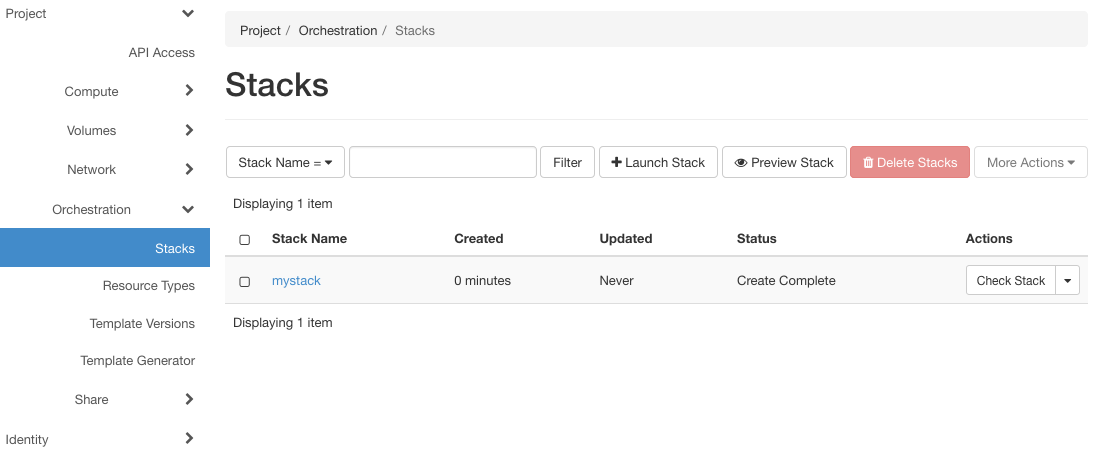
\includegraphics[width=\textwidth]{img/stacks_overview}
\end{center}
The overview page contains a list of all currently existing stacks
(either running or suspended), and buttons to perform the following
actions:

\subsection*{Launch a stack}
\begin{enumerate}
\item Click \strong{Launch Stack} to open the following wizard:
\begin{center}
  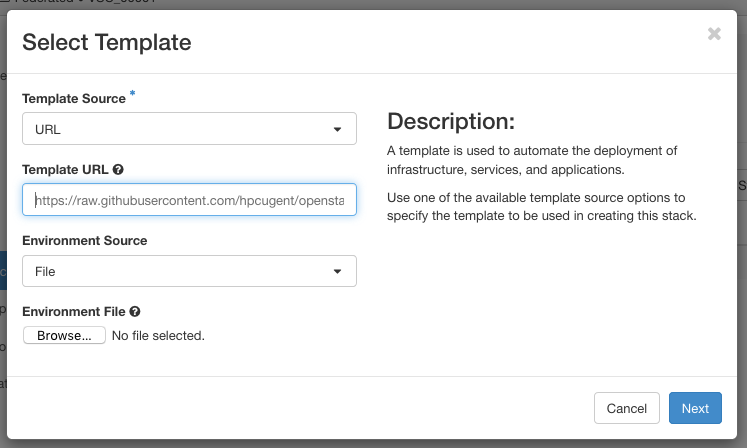
\includegraphics[width=0.7\textwidth]{img/launch_stack_template}
\end{center}
\item Provide a template and --- optionally --- an environment for the stack.
\begin{description}
\item[Template Source] You can provide a template using one of the
  following options:
  \begin{description}
  \item[File] Provide a local file on your system.
  \item[Direct Input] Enter the template in a text field.
  \item[URL] Provide a \textsc{URL} to have OpenStack download the
    template from that location.
  \end{description}
  In our example, we provide a \textsc{URL} from the repository
  \href{https://github.com/hpcugent/openstack-templates}{github.com/hpcugent/openstack-templates},
  to instantiate the example from section \ref{sec:glsh-orch-templ}.
  If you want to provide a template directly from GitHub, make sure to
  provide a ``Raw'' \textsc{URL},
  \lstinline{https://raw.githubusercontent.com/}\ldots.

\item[Environment Source] Optionally, you can also provide an
  environment file.  This is another \textsc{yaml} file, which
  contains customizations for your Heat templates, such as default
  values for parameters, or custom resource types you have created
  (see
  `\href{https://docs.openstack.org/heat/\osversion/template_guide/environment.html}{Environments}'
  in the Heat template guide).  You can provide a \strong{File} or
  choose \strong{Direct Input}.
\end{description}
\item If you click \strong{Next}, OpenStack will process the template.
  You can now enter a name for the stack, and provide values for all
  the template parameters:

  \begin{center}
    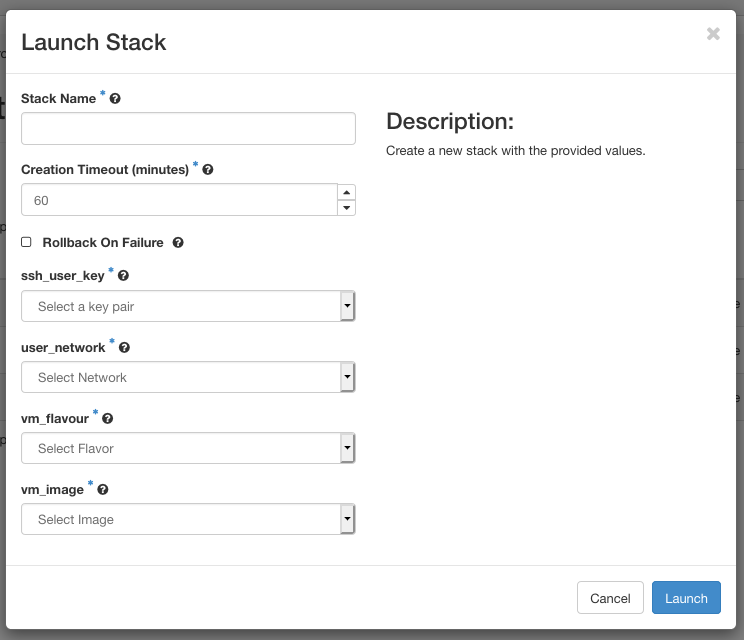
\includegraphics[width=0.7\textwidth]{img/launch_stack_parameters}
  \end{center}
\item Click \strong{Launch} to instantiate the stack.
\end{enumerate}

\subsection*{Preview Stack}
\strong{Preview Stack} starts a wizard similar to the ``Launch Stack''
wizard, but completing the wizard will only make the system perform a
sanity check of your template, without instantiating the stack.  If
the check passes, you can inspect the parameters of the stack that
would be created.  The wizard does not allow you to enter input
parameter values, so any mandatory input parameters should be provided
in an environment.

\subsection*{Delete Stacks}
\strong{Delete Stacks} deletes all selected stacks from the list .

\strong{Warning:} Deleting a stack also deletes all of the resources
(volumes, ports) created by that stack, unless a different policy was
set in the \strong{\lstinline{deletion\_policy}} property for those
resources (see the
`\href{https://docs.openstack.org/heat/\osversion/template_guide/hot_spec.html#resources-section}{Resources
  section}' in the \textsc{hot} specification).

\subsection*{More Actions}
The button \strong{More Actions} hides the following additional
actions:

\begin{description}
\item{\strong{Check Stacks}} verifies if the resources for selected
  stacks are still running.
\item{\strong{Suspend Stacks}} suspends all resources of the selected
  stacks.
\item{\strong{Resume Stacks}} resumes the selected (suspended) stacks.
\end{description}

You can quickly suspend, resume or delete a single stack using the
drop-down menu in the \strong{Actions} column of the overview.  This
menu also contains the option \strong{Change Stack Template}, which
allows you to update a Stack by providing a new template.

%%% Local Variables:
%%% mode: latex
%%% TeX-master: "intro-Cloud"
%%% End:
